\documentclass[../main.tex]{subfiles}
\begin{document}
	In the medium with normal dispersion, for input peak power between
	$P_{cr}$ and $P_{th}$, beam collapse, caused by self focusing, is
	prevented by dispersion. To characterise GVD regime more clearly, we
	defined two characterstic lengths.
	First one is the \textbf{self focusing length ($z_{sf}$)}, which is
	distance at which collapse of beam should occur in absense of other
	mechanism.
	\begin{equation} \label{eq:self_focusing_len}
		z_{sf} = \frac{0.183 \rho_0}
		{\sqrt{\left( \sqrt{P_0 / P_{cr}} - 0.852 \right)^2 - 0.0219}}
	\end{equation}
	Where $\rho_0 = \frac{\pi w_0^2 n_0}{\lambda}$.
	The other characterstic length is the propagation distance over which
	input peak power got reduced to critical power due to combine effects of
	GVD and SPM.
	\begin{figure} [h]
		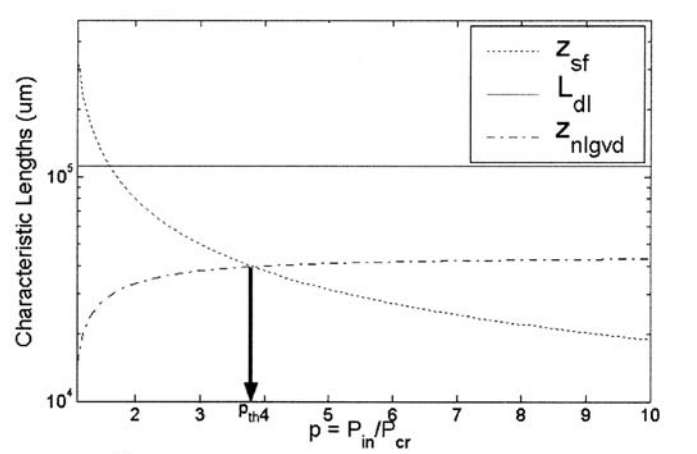
\includegraphics[width=0.5\textwidth]{images/len.png}
		\caption{Characterstic lengths for GVD, for BK-7
		\label{fig:char_len}}
	\end{figure}
	\begin{equation} \label{eq:gvd_len}
		z_{nlgvd} = 0.5\rho_0 \left[ \frac{\sqrt{3.38 + 5.2( (P_0 /
			P_{cr})^2 - 1)} - 1.84}
			{15(P_0 / P_{cr}) \gamma} \right]^2
	\end{equation}
	Where $\gamma = \rho_0 / L_{dl}$ and $L_{dl} = t_0^2 / 2\beta_2$ is
	dispersion length. Both these characterstic lengths are plotted in
	fig~[\ref{fig:char_len}] along with dispersion length.
	Input power at which both these lengths are same is our threshold power
	($P_{th}$). For BK7, $P_{th} = 3.85 P_{cr}$.
	\begin{figure} [h]
		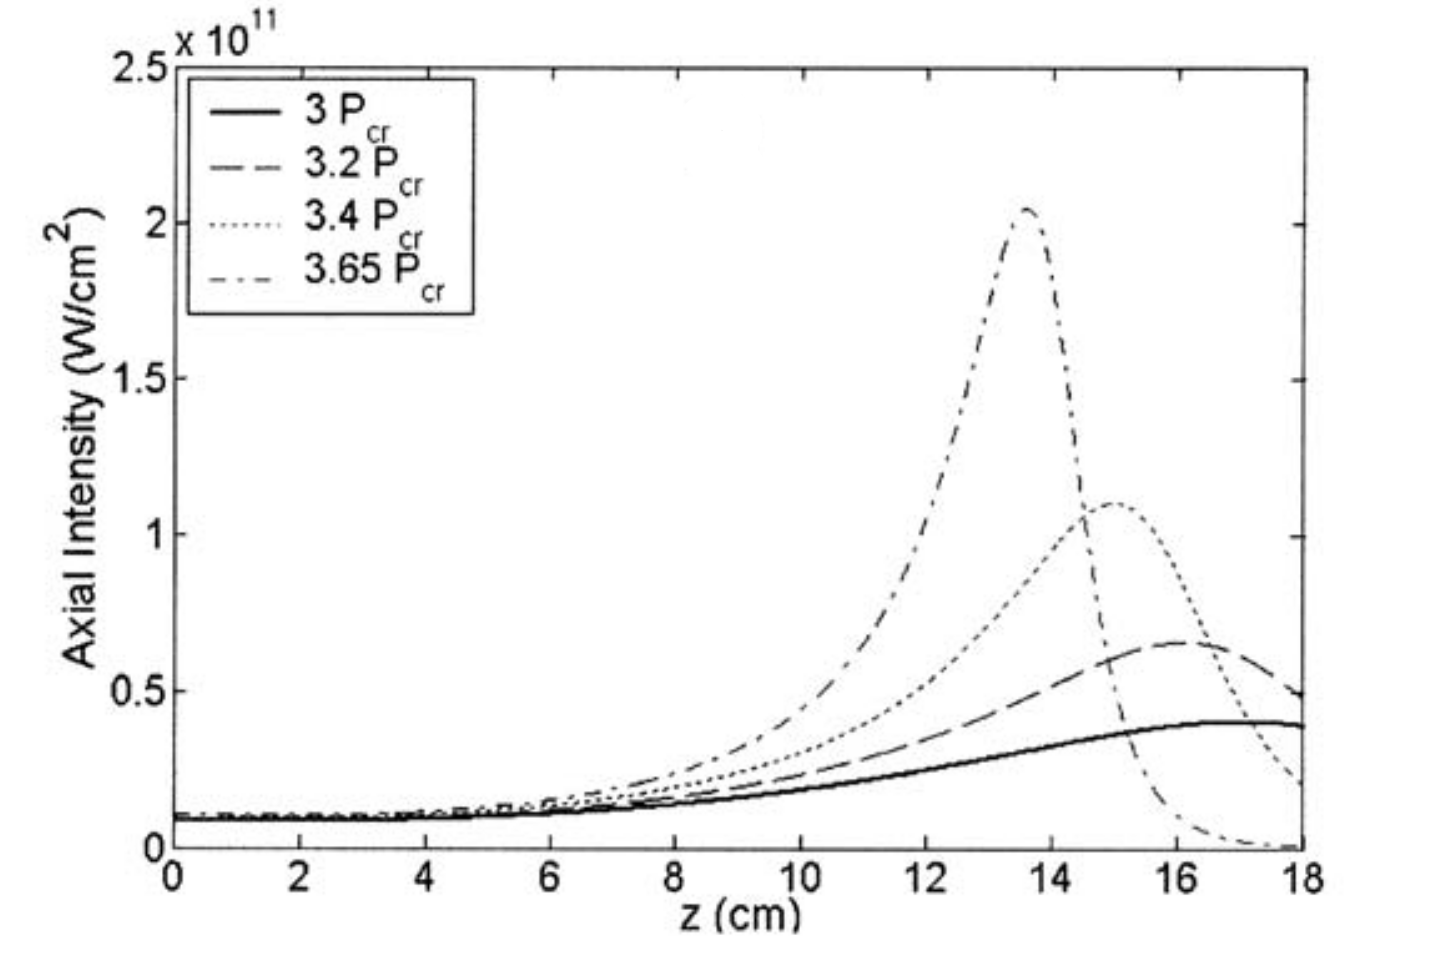
\includegraphics[width=0.5\textwidth]{images/gvd.png}
		\caption{Variation of axial intensity with propagation distance,
			z, for various input power ranging from $P_{cr}$ to
			$P_{th}$.
		\label{fig:inten_gvd}}
	\end{figure}

	\begin{figure} [h]
		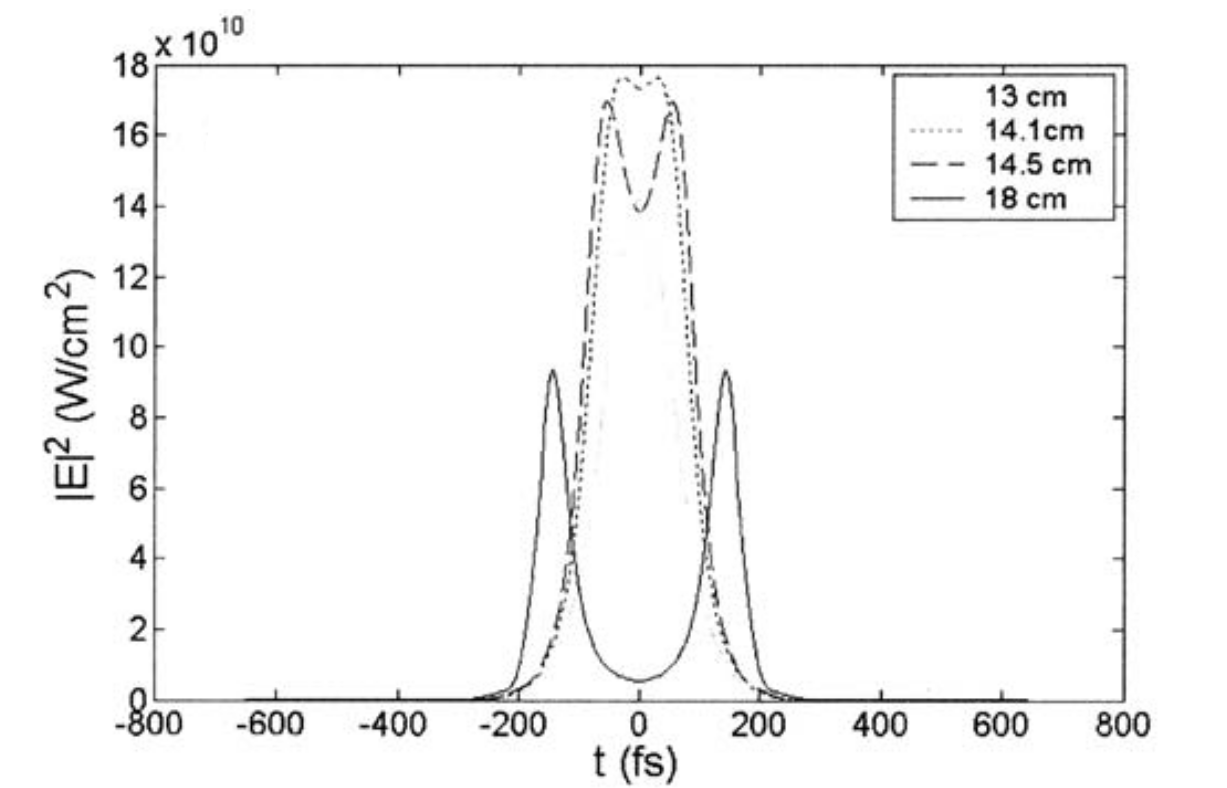
\includegraphics[width=0.5\textwidth]{images/split_gvd.png}
		\caption{Temporal splitting at nonlinear focus for $P_{th}$.
		\label{fig:split_gvd}}
	\end{figure}
	Figure [~\ref{fig:inten_gvd}] shows peak getting higher and advancing
	towards entry of medium as input power increase. In this regime,
	collapse of pulse is prevented by pulse broadening and splitting. Pulse
	broadening happen due to dispersion.

	Combination of self focusing and SPM induce pulse splitting. At $t=0$,
	self focusing pushes off-axis energy towards the centre of pulse. As
	peak intensity increases due to self focusing, SPM start generating new
	frequencies. This introduce a chirp along the pulse. The up and down
	shifted pulses increase in intensity and get end up splitting due to
	normal dispersion. See figure [~\ref{fig:split_gvd}].
\end{documents}
